\documentclass[review]{elsarticle}

\usepackage{lineno,hyperref}
\modulolinenumbers[5]

\usepackage[margin=1in,nohead]{geometry}
\usepackage{amsmath}
\usepackage{amssymb}
\usepackage{makecell} %Table text splitting

\journal{Energy Strategy Reviews}

%%%%%%%%%%%%%%%%%%%%%%%
%% Elsevier bibliography styles
%%%%%%%%%%%%%%%%%%%%%%%
%% To change the style, put a % in front of the second line of the current style and
%% remove the % from the second line of the style you would like to use.
%%%%%%%%%%%%%%%%%%%%%%%

%% Numbered
\bibliographystyle{elsearticle-num.bst}

%% Numbered without titles
%\bibliographystyle{model1a-num-names}

%% Harvard
%\bibliographystyle{model2-names.bst}\biboptions{authoryear}

%% Vancouver numbered
%\usepackage{numcompress}\bibliographystyle{model3-num-names}

%% Vancouver name/year
%\usepackage{numcompress}\bibliographystyle{model4-names}\biboptions{authoryear}

%% APA style
%\bibliographystyle{model5-names}\biboptions{authoryear}

%% AMA style
%\usepackage{numcompress}\bibliographystyle{model6-num-names}

%% `Elsevier LaTeX' style
%\bibliographystyle{elsarticle-num}

%% `Elsevier LaTeX' style
%\bibliographystyle{elsarticle-harv.bst}
%%%%%%%%%%%%%%%%%%%%%%%

\begin{document}
\begin{frontmatter}

\title{Characterizing Fusion Market Entry via an Agent-based Power Plant Fleet Model}

%% use optional labels to link authors explicitly to addresses:
%% \author[label1,label2]{}
%% \address[label1]{}
%% \address[label2]{}

\author[lucas]{Lucas Spangher\corref{}}
\author[scott]{J.Scott Vitter}
\author[ryan]{Ryan Umstattd}
\address[lucas]{Corresponding author.  U.S. Department of Energy Advanced Research Projects Agency -- Energy (ARPA-E), e-mail: \url{lucas_spangher@berkeley.edu}, fax: +1 (510) 643-7846. Currently at the University of California, Berkeley.}
\address[scott]{The University of Texas at Austin, e-mail: \url{scott.vitter@utexas.edu.}}
\address[ryan]{U.S. Department of Energy Advanced Research Projects Agency -- Energy (ARPA-E), \url{Ryan.Umstattd@hq.doe.gov}}

\begin{abstract}
An agent based model characterizing the U.S. power plant fleet was formulated to compare scenarios for fusion energy technology diffusion. The model employs historical data to form distributions for power plant retirements, and simulates construction of new capacity to meet electricity demand on an annual basis. Scenario analysis within this paper explores model sensitivity to 1) the year of market entry for commercial fusion technologies, 2) rate of diffusion, and 3) market capture limit. Results indicate that the first-decade market potential for fusion power plants depends on retirements of other generating resources and finds that near-term availability of fusion technology has limited potential to mitigate fleet-wide emissions in the near term, even at high rates of market capture.  
\end{abstract}

\begin{keyword}

Agent-based modeling \sep Fusion Energy \sep Power Plant \sep Green New Deal 
%% keywords here, in the form: keyword \sep keyword
%% PACS codes here, in the form: \PACS code \sep code
%% MSC codes here, in the form: \MSC code \sep code
%% or \MSC[2008] code \sep code (2000 is the default)

\end{keyword}
\end{frontmatter}

\section*{Highlights}
\begin{itemize}
\item Fleet inertia limits the pace for impacting total carbon emissions
\item Initial market opportunity for fusion is dominated by plant retirements 
\item Initial market opportunity for fusion is weakly dependent on year of market entry
\item Early availability and deep market capture  are required for fusion technology to significantly extend a nominal CO$_2$ emissions budget. 
\item The first implementation with respect to nuclear fusion of the longer term decarbornization envisioned in the Green New Deal is presented. 
\end{itemize}

\section*{Glossary}
The following abbreviations are used throughout this paper:

\begin{itemize}
\item ALPHA - Accelerating Low-Cost Plasma Heating and Assembly
\item BAU - Business as Usual
\item EIA - Energy Information Administration 
\item GHG - Greenhouse Gas 
\item Fusion - Nuclear Fusion 
\item Nuclear - Nuclear Fission
\item NGCC - Natural Gas Combined Cycle
\item NGCT - Natural Gas Combined Turbine
\item NGST - Natural Gas Steam Turbine
\item PV - Photovoltaic
\end{itemize}

\section{Introduction}
The electric power sector is a major source of greenhouse gas (GHG) emissions in the United States, contributing 29\% of all GHG emissions in 2015, ahead of transportation (27\%)\citep{EPA2017}. To achieve deep decarbonization across the entire economy, the electricity sector must eventually shift to near-zero emission generation technologies.

Nuclear fusion has been proposed as a potentially transformational technology to provide abundant, sustainable, reliable, and carbon-free electricity generation \citep{Chou2016}. In a fusion reaction, nuclei combine in an exothermic reaction, giving off heat that can be the source for a thermal power plant \citep{Chou2016}. Several fusion fuel cycles have been researched, and they share many potential advantages: The hydrogen isotope deuterium (2H) is naturally occurring; reactors can be engineered to breed additional tritium (3H) to fuel future reactors; waste streams from fusion byproducts will be less hazardous than nuclear fission byproducts; operational risk can be greatly reduced relative to nuclear fission; and fusion power plants have the potential to operate reliably and controllably \citep{Chou2016}. To be acceptable to electric utilities, fusion power plants must meet several key criteria including low electricity costs, public acceptance, and a simple regulatory review process \citep{Kaslow1994}.

Even with early commercialization of fusion technology, however, altering the composition of the generating fleet could be difficult.\citep{Tokimatsu2002} Capital requirements for new power plants are high, and new power plants typically operate for decades. The electricity sector's technological inertia is exemplified by the capacity-weighted average lifetime of domestic power plants, which in 2016 was approximately 54 years \citep{EIA2016}. Given these barriers, this paper addresses how the generation fleet in the US might evolve if fusion energy achieves technical feasibility and public acceptance. An agent-based model was built to represent the U.S. power plant fleet on a granular level, using historical data for power plant lifetimes, retirements, and future projections for electricity demand. Parameters including year of entry, diffusion rate, and fraction of annual market capture are varied to determine their influence on the future composition of the generation fleet and the trajectory of carbon emissions from the power sector from 2017 to 2100. To characterize the impact of technological breakthrough in fusion, market entry scenarios begin in 2030. Overall, modeled scenarios suggest upper bounds for installed capacity and carbon emission reductions attributable to fusion energy.

In the U.S., recent policy discussions motivate our work. The Green New Deal (GND) has generated momentum to enact decarbonization policies in many energy sectors, including electricity. For electrical power, the GND calls for ``meeting 100 percent of the power demand in the U.S. through clean, renewable, and zero-emission energy sources.'' \citep{GND2019} We outline scenarios in this paper that, in part, consider the effects of such a policy being passed. For this reason, we believe our paper is uniquely relevant to current policymakers and helps assess the feasibility of such ambitious targets. To our knowledge, this is the first quantitative outline of technological pathways to help the electricity goals of the Green New Deal to be realized as nuclear fusion is concerned.

\section{Background}

Forecasting the evolution of the power generation fleet is an active area of research in the energy community. Prominent models include the National Energy Modeling System (NEMS), which is an integrated energy-economy model of U.S. energy markets extending through 2050 \citep{AEO2017}. NEMS is employed by the Energy Information Administration (EIA) to project the evolution of the generation fleet in its Annual Energy Outlook (AEO) reports \citep{NEMS2014}. The National Renewable Energy Laboratory (NREL) has formulated a Regional Energy Deployment System (ReEDS) model, which is a long-term capacity model for the deployment of generation technologies and transmission infrastructure in the United States \citep{ReDS2016}. ReEDS is an optimization model that solves for a mix of generating technologies to meet constraints relating to technology, resources, electricity demand, reliability, and policy. A model generator developed by the Energy Technology Systems Analysis Programme (ETSAP) of the International Energy Agency, MARKAL, was formulated as a dynamic linear program to resolve energy systems \citep{Fishbone2981}. MARKAL has given rise to TIMES, a hybrid model generator meant to explore energy futures [24]. In general, these models have been employed to forecast the evolution of conventional energy technologies, excluding fusion power plants [24]. One exception is the Global Change Assessment Model (GCAM) model, developed and maintained by the Pacific Northwest National Laboratory, which is an integrated assessment model that has been applied to a limited set of fusion scenarios \citep{Chou2016} \citep{ACFD}. Other papers have also explored the long-term potential for fusion power, finding significant long-term potential if assumptions for capital costs are realized \citep{Fishbone2981} \citep{Gnansounou2007} \citep{Han2009} \citep{Cook2002}.

Related work in this field has explored the spread of new technology, dating back to original research by Griliches \citep{Grilliches1957}, who established in 1957 s-curves as a model of technology diffusion. First introduced by epidemiologists to describe the spread of disease in a population, the s-curve has been used throughout numerous anthropocentric fields as a method to model human behavior \citep{Sovacool2016}. The formulation of s-curves has been extensively studied, including an extension by the Bass model to study new consumer electronics \citep{Bass1969}. Diffusion of innovations is an area of ongoing research involving s-curves \citep{Kijek2015}, which has been applied to fields such as epidemiology \citep{Wang2011} and energy technology adoption \citep{Schilling2008}.

Many models of the electricity sector are top-down, meaning that they attempt to summarize the entire economy by using separate modules that interact with each other in complex ways. A high degree of granularity is required to model the addition and retirement of individual generator assets, which is a primary objective in this study. Agent-based modeling (ABM) is an emerging field that can help understand electricity market dynamics. A set of agents is used to represent social actors, imbued with simple decision-making rules, in an environment where agents interact following rules and limitations present in the real world \citep{Gilbert2008}.  ABM allows the behavior of individuals to be easily modeled, enabling the behavior of the aggregate group to be analyzed. Weidlich and Veit \citep{Widlich2008} give a review of ABM relevant to the electricity sector.

The electricity sector is comprised of few enough components that an agent-based model can summarize it with near-perfect granularity: one agent per one real-world power plant. A first-order ABM approach, independent of costs, can determine the upper bound for diffusion of new technology. To study the effects of fusion power plant entry year, diffusion, and market capture, an ABM approach was formulated using historical distributions for power plant retirement by generation technology. The model described in this paper allows for simulations of wide-ranging and long-term fusion scenarios, and it can help explore the market potential for fusion power plants given the lifetime, retirement, and new construction of competing technologies.

\section{Model Development}

Section 3.1 - 3.5 describe agent creation, detail the assignment of power plant lifetime or retirement age, explain model estimations of future electricity demand, and lay out processes to simulate retirements and additions of new capacity. Section 3.6 summarizes the scenarios that underlie the results of the paper.

\subsection{Agent Creation}

The United States Energy Information Agency (EIA) maintains a historical inventory of electricity generating units with a nameplate capacity exceeding one megawatt \citep{EIA2016}. This dataset consists of the current fleet, planned new additions, and units that were previously retired. In addition to capacity, each entry is annotated by its first year in operation as well as the primary, secondary, and tertiary energy source; technology (e.g. steam turbine, combustion turbine, combined cycle, internal combustion engine, photovoltaics, wind turbine); current age; and latitude/longitude of power plant location.

An agent-based model was created to match the fleet of electric power plants in the United States circa 2015. A power plant agent pi was created to match each entry in the EIA dataset a capacity greater than 1 MW, so the agents closely resembled the generation fleet in the United States at the start of the simulation. Each plant was assigned an operating capacity (MW) and capacity factor based on historical EIA data. Emissions factors ($frac{kg CO_2}{kWh}$) were also assigned based on the primary fuel type \citep{EIA_1605_2016}. This information is presented in Table 1.

\subsection{Retirement age assignment}

Each agent $p_i$ was assigned an expected retirement age that was determined probabilistically by forming distributions of past retirement ages for each type of power plant \citep{EIA2016}. Skewed normal distributions were then fit to these sample distributions. EIA data for retirement age distributions were sparse for some technologies. For example, retirement age data is limited for wind farms and solar PV installations because 99\% of the installed capacity in the United States has been built since 2000. To overcome these limitations, skewed distributions were assumed to reflect a median lifetime of 25 years for wind, PV, solar thermal, and municipal solid waste generators. Nuclear power plants retire upon expiration of their operating license from the Nuclear Regulatory Commission (NRC). This study assumed that two-thirds of the nuclear fission plants were granted a 20-year extension past the 40-year initial license, for a total lifetime of 60 years, while one-third retire at 40 years. Each agent's retirement age was then determined by sampling the applicable distribution. New fusion power plants built by the model are assigned a lifetime of 40 years.

\subsection{Electricity demand and new capacity growth}

One goal of the model was to evaluate market penetration by novel fusion technologies up until 2100, which required a forecast for annual electricity demand from the grid. The trajectory of future electricity demand is uncertain, but the EIA's Annual Energy Outlook 2017 \citep{NEMS2014} forecasts near-linear electric demand growth from approximately 4,000 terawatt hours (TWh) in 2015 to approximately 4,700 TWh in 2050. The AEO includes forecasts for capacity growth by power plant type. To extend the model through 2100, baseline scenarios in this paper assumed continued demand growth, eventually reaching approximately 6,200 TWh in 2100. The model can be deployed for other demand scenarios where electricity demand remains roughly constant or decreases into the future, which can help quantify uncertainty associated with the proposed model. \citep{Cook2002}

The AEO 2017 also forecasts new capacity on the grid by technology type for each year between 2016 and 2050 \citep{NEMS2014} . Renewable energy is expected to make up the bulk of new capacity additions, followed by natural gas combined cycle and combustion turbine power plants \citep{NEMS2014} . The relative fraction of new capacity in year t for technology $j_{t,j}$, is used by the model to introduce new power plant agents to replace retiring capacity, and will be discussed in subsequent sections. Notably, scenarios evaluated in this study do not consider scenarios where new coal, nuclear fission, solar thermal, biomass, or municipal solid waste capacity is added as we consider these scenarios either very improbable or with too small an addition to make a difference.

The AEO uses an underlying model called the National Energy Modeling System (NEMS), which is an integrating model seeking to endogenously incorporate interactions between economic changes, energy supply, demand, and price. Thus, although price does not explicitly drive choices in the model, it is implied through the relationship to the AEO projections. As AEO incorporates these dynamics into its model, the same price related dynamics that affect its future energy supply are implied in our model. 

\subsection{Annual retirements/additions of new power plant agents}

The model wraps all aforementioned components in a Markov chain to simulate time dependency: 
$$ p(x_t|x_{t-1})=p(x_{t-1},x_{t-2},...,x_1)\neq p(x_t)$$

Where $x_i$ are general states of the scenario. The Markov chain has yearly time steps from 2014 to an exogenous end year. During each time step, the model retires all power plant agents whose age exceeds their life expectancy. Following retirements, the model calculates a shortage $S_t$ of electricity (in MWh) in year t to be met by new power plant additions:

$$S_t=E_{t,proj}- \sum_{i=1}^M(p_{i,cap}*p_{i,CF}*8760)$$ 

Where $E_{t,proj}$ is the projected net electricity demand, $i$ identifies the power plant, $p_{i,cap}$ is power plant capacity, and $p_{i,CF}$ is annual capacity factor. To meet the electricity shortage caused by power plant retirements, the model simulates adding new capacity. Based on plant type, new power plant agents are assigned a capacity, capacity factor, and emissions characteristics as calculated from AEO 2017 data and shown in Table 1. Each set of new agents for a given generation technology is assumed to be homogeneous, so characteristics such as capacity factor do not vary within the category. Each new plant is also assigned a lifetime in the manner described previously (Section 3.2). Fusion power plants were assigned a mean capacity of 500 MW under the assumption that while the market may prefer smaller, more modular, less capital-intensive power plants, there will be economies of scale for tritium and neutron handling that will push fusion towards larger plants. Fusion was assigned a capacity factor of 0.75, which balances an expectation that fusion will run continuously with challenges associated with maintaining power plants based on new technology.

\begin{table}[!htbp]
	\centering
	\scriptsize
	\caption{For each type of power plant represented in the model, values were defined for mean plant capacity, capacity factor, marginal emissions, and embodied emissions [1, 21].  *MSW is abbreviated Municipal Solid Waste}
	\label{tab_embod}
	\begin{tabular}{lllll}

Technology & Mean Plant Capacity (MW) & Average Capacity Factor & Marginal Emissions ($\frac{kg CO_2}{kWh}$) & Embodied Emissions ($\frac{kg CO_2}{kWh}$) \\ \hline \hline
Biomass &20 & 0.53 & 0.39 & 210 \\ 
Coal & 280 & 0.54 & 0.33 & 10\\
Geothermal & 20 & 0.72 & 0.03 & 45\\
Hydroelectric & 20 & 0.36& 0 & 19 \\
MSW* & 30& 0.68 & 0.14 & 2 \\
NGCC & 140 & 0.56 & 0.18 & 2 \\
NGCT & 60 & 0.07 & 0.18 & 2 \\
NCST & 150 & 0.12 & 0.18 & 2 \\
Nuclear & 1050 & 0.92 & 0 &  18\\
Petroleum & 13 & 0.1 & 0.25 & 10\\
PV & 7 & 0.29 & 0 & 66\\
Wind &  60 & 0.33 & 0 & 15 \\
Fusion & 500 & 0.75 & 0 & 18\\\hline
	\end{tabular}
\end{table}

Because the average capacity factor of power plant technologies varies, a weighted capacity factor of new generation is used to determine the breakdown of new agent assignments in a given year. The assignment of $\alpha_{t,j}$ is exogenous, and is defined by the scenario of interest:
$$ CF_{t,new} = \sum_{j \in J} \alpha_{t,j} \bar{CF_{j}}$$ $$N_t=\frac{S_t}{CF_{t,new}}$$ 
$$n_{t,j} = \frac{N_{t,j}}{C_j}$$

Where $CF_{t,new}$ is the weighted capacity factor of new capacity additions in year $t$, $CF_j$ is the capacity factor of power plants of type $j$, $\alpha_{t, j}$ is the fraction of new capacity from technology $j$ in year $t$, $N_{j,t}$ and $N_t$ are the amounts of technology-specific and total new generation capacity allotted in year $t$, and $C_j$ is the capacity of new power plants of type $j$. Depending on the type of power plant and the quantify of allocated capacity, $n_{t,j}$ new plants of type $j$ are added in year $t$. Because a fraction of a plant cannot be added, $n_{t,j}$ is rounded down to the nearest integer and can assume a value of zero.

For the business-as-usual baseline scenario without fusion power plants, values for $\alpha_t$, are taken from AEO projections. For scenarios with fusion power plants, the new capacity fractions for non-fusion technologies are reduced in proportion to the prevalence of fusion power plants. Once technology-specific capacity additions are calculated, the model adds new power plant agents to the fleet. Agents are assigned capacities according to Table 1 and life spans are assigned according to the sampling procedure previously described. 

Once the fleet is assembled, the model calculates annual greenhouse gas emissions according to average emissions factors from Table 1 \citep{IPCC2012}. The model then advances in time, retires power plants in year $t+1$, and continues with the previously described steps. Simulated electricity generation by the model matches the forecasted net load, but capacity installations depend on the average capacity factor of the technologies built by the model. For example, building more wind and solar in place of coal will result in more installed capacity overall because the average capacity factors of wind and solar resources are less than the average capacity factor of coal plants.

\subsection{Timed entry and diffusion of learning for fusion power plants}

In the modeled baseline scenario, fusion power plants do not appear in the model, reflecting a future where fusion power plants are never commercially viable. Subsequent scenarios evaluate the power plant fleet for various combinations of fusion entry year, market capture, and technology spread. For this analysis, a modified version of the s-curve determines the trajectory of fusion plant market capture from zero to $p_{ceil}$, where $p_{ceil}$ is the maximum percentage of yearly new electricity capacity comprised of new fusion plants: 

$$p_t = \frac{p_{ceil}}{1+e^{-(a_0+a_1t)}}$$

Where $p_t$ is the percentage of new electricity capacity from fusion in year $t$. The parameters $a_0$ and $a_1$ are exogenous, representing the year that fusion technology becomes commercially viable and the duration of the technology spread period. In this formulation, the fusion market capture increases monotonically, traveling up the s-curve each year independent of how many power plants are built. The form of the s-curve is unbounded and asymptotes at both 0 and $p_ceil$, so $I_ceil$ is introduced to allow specification of the duration in years required for new fusion capacity to increase from 5\% to 95\% of pceil. $I_ceil$ influences the s-curve by exogenously influencing $a_1$:

$$a_1 = \frac{\log(19)-\log(\frac{1}{19})}{I_{ceil}}$$

The model was used to investigate the impacts of choosing 5, 10, 20, or 30-year durations for this s-curve, with little net change in the overall characteristics of the result except for scenarios with very high fusion penetrations. A 10-year s-curve, consistent with modern regional energy transitions \citep{Sovacool2016}, was assumed for subsequent results.

\subsection{Summary of scenarios}

An illustrative case description was carried out by varying the year of fusion market entry (2030, 2050, 2070) and the duration of technological diffusion in years (10, 20, 30). In addition, we vary the maximum rate of market capture on an annual basis (10\%, 50\%, 99\%); this design decision was made as a proxy to consider a range of potential cost considerations for yet-to-exist fusion power plants, with the lowest expressing the least cost competitiveness and the higest expressing the most. This scenarios form a spectrum, from early entry and aggressive growth to delayed entry with moderate adoption, to help understand the range of potential outcomes should fusion technology meet criteria for utility acceptance in the United States \citep{Kaslow1994}. We believe that scenarios with the highest parameters are useful and relevant when considering the speed at which clean sources of energy are to be implemented in the Green New Deal in the United States. 

Finally, the scenarios presented in this paper do not include several potential competitors to fusion, including carbon capture and sequestration and advanced nuclear fission technologies. Including these technologies into the ABM is an area for future work. Because candidate technologies are excluded in the present analysis, modeled results are considered an upper bound for fusion penetration.

\section{Results and Discussion}

Results from model simulations of scenarios with 10\% deployment and 50\% deployment are presented and discussed to demonstrate capabilities of the model and investigate the potential for fusion technology to capture electricity generation market share and impact total emissions.  We believe the scenario analysis we construct is aligned with recent trends in the U.S., especially considering recent policy momentum generated by the Green New Deal.  The section is organized as follows: In Section 4.1, model projections for fleet wide evolution are examined for a range of scenarios including fusion power plants. In Section 4.2, the market opportunity for fusion power plant technology is explored in a parameter study. In section 4.3, scenarios are compared to evaluate U.S. power plant fleet emissions trajectories with and without the presence of fusion energy technology. Two additional sections, inserted in the appendix, provide model validation. Section 4.1 compares model predictions to forecasts published by the EIA through 2050. Section 4.2 examines a business-as-usual case where fusion power plants do not enter the market before 2100 and retired capacity is replaced by a mix of primarily renewables and natural gas power plants. 

\subsection{Fleet-wide capacity evolution with fusion power plant entry}

The generation mix of installed capacity in the model depends on the entry year of fusion technology, its maximum percentage of new power plant market capture, and the modeled s-curve, which dictates how quickly the maximum market capture is reached. When fusion becomes commercially available to the model, market share captured by competing technologies such as NGCC and renewables is proportionately reduced.

Figures 1.a through 1.f demonstrate how the technology mix among the generation fleet can influence total installed capacity on the grid. For example, in Figure 1.e, future load growth is primarily met by NGCC and renewables, which reduces the fleet-wide capacity factor in the model, resulting in growth of total installed capacity from approximately 1 TW in 2015 to 1.3 TW in 2075. Conversely, the model predicts that overall installed capacity on the U.S. grid would decrease to 900 GW in 2075 if fusion power was available by 2030 and was added to capture half of the newly installed capacity each year. In this study, fusion power plants have an assumed capacity factor of 0.75, so building fusion power plants increases the fleet-wide average. Because the model does not consider hourly or sub-hourly unit commitment and dispatch, second-order effects relating to grid reliability, reserve procurement, and ancillary service procurement are not quantified by the model. Qualitatively, if the grid evolves by decreasing installed capacity, the remaining power plants must be capable of flexible operations that allow grid operators to balance electric supply and demand, perhaps requiring energy storage to satisfy hours of peak electric demand. If the grid evolves to be dominated by non-dispatchable renewable resources, storage technology capable of daily or even seasonal load shifting might be required to balance electricity supply with demand.

Retirements of the existing coal-fired and nuclear fleet could be considered an opportunity for fusion power plants to enter the market and provide baseload power before 2050. Figures 1.a-1.b indicate how the model expects the generation mix to evolve in near-term scenarios as coal or nuclear units approach the end of their lifespan and are not replaced. From 2020 to 2050, the modeled capacity of coal-fired units decreases from 232 GW to 47 GW. Installed capacity of the nuclear fleet decreases from 94 GW to 11 GW over the same period. Beyond 2050, the retirements of remaining plants slow, with installed capacity of both technologies dropping below 1 GW in approximately 2080. In Figure 1.a, fusion technology that enters the model at 2030 and ramps up production to capture 10\% of new generating capacity in ten years (2030-10\% case) installs 52 GW on the grid by 2050, which is only 15\% of the 338 GW of coal and nuclear retired by the model from 2015-2050. The majority of retirements in Figure 1.a before 2050 are replaced by NGCC, wind, and solar generation, although hydro and NGCT remain a significant part of the installed generator mix. Conversely, fusion technology entering the market in 2030 (Figure 1.b) and ramping up to eventually meet 50\% of new capacity would build 190 GW of fusion capacity on the grid by 2050. 

Clearly, a scenario such as the one presented in Figure 1.b is superior when considering the impact that fusion might have on long term decarbonization of the grid considered in the Green New Deal. However, given the latency in power plant turnover, we advocate the pairing of fusion with other technologies in the implementation of the Green New Deal.

\begin{figure}
\begin{center}
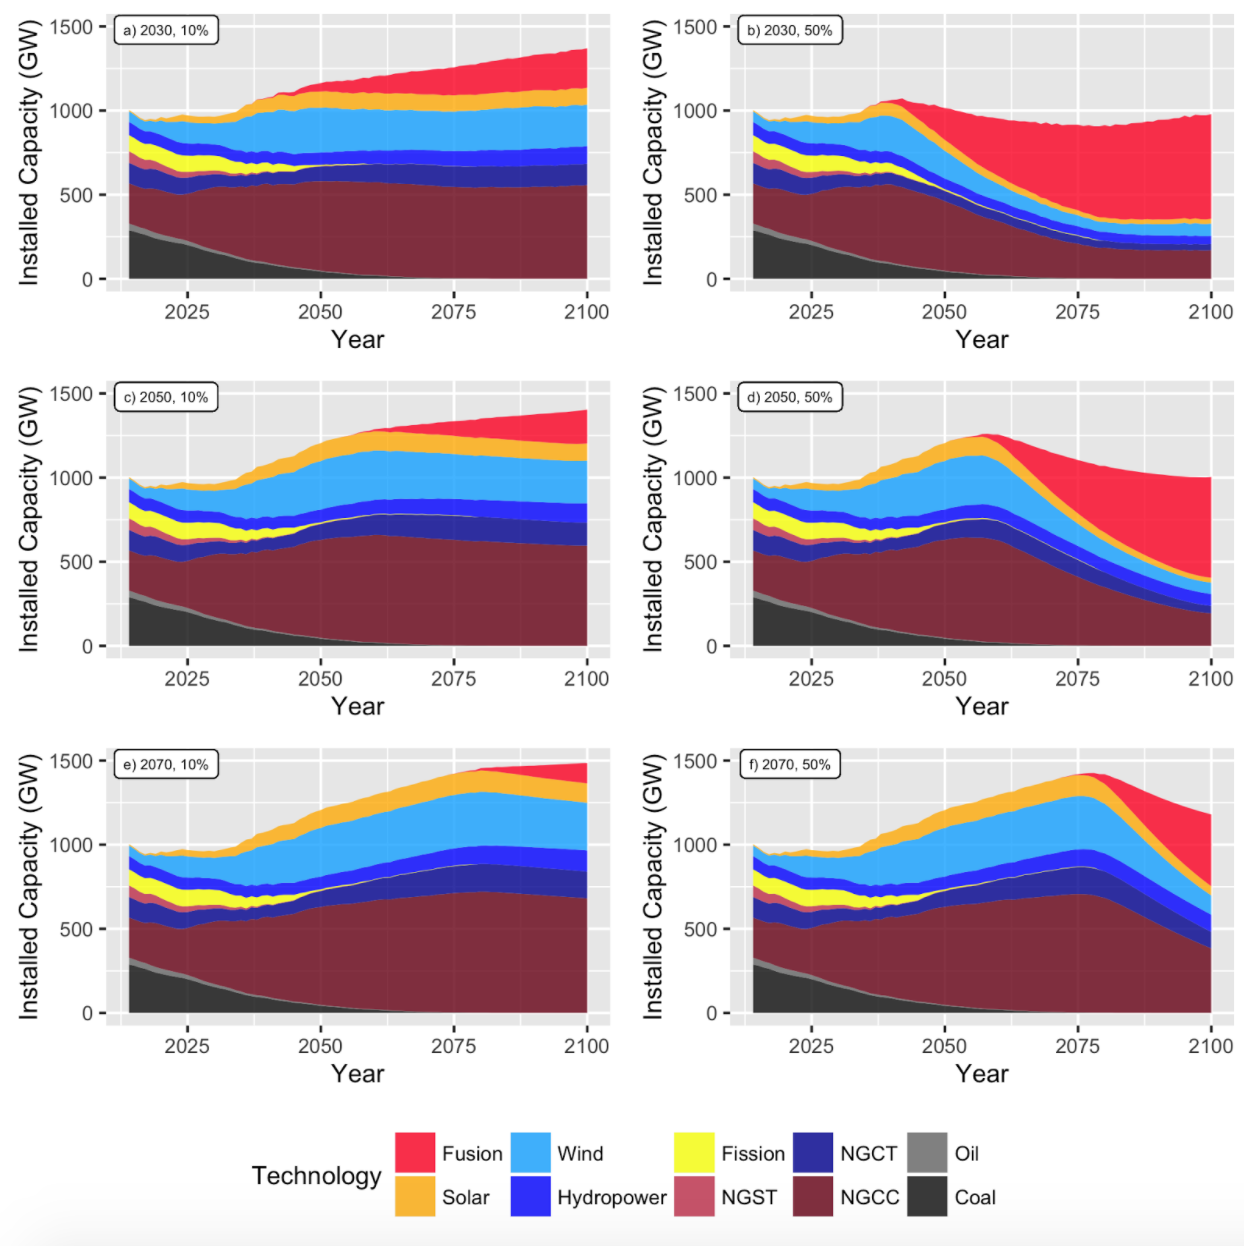
\includegraphics[width=\textwidth]{mainFig.png}
\end{center}
\caption{Installed capacity by technology type for different entry dates and market capture ceilings for fusion power plants. These figures help visualize the market opportunity for fusion power plants based on when the technology is available relative to retirements and growth occurring in the existing fleet.}
\end{figure}

In Figure 1.c through 1.f, fusion technology does not become commercially viable until only small amounts of coal and nuclear remain on the grid. The opportunity for fusion is limited to competing for new demand growth and replacing retiring NGCC, wind, and solar facilities. 

Another result from the fleet-wise visualization is that growth in installed capacity for wind and solar resources slows beyond 2050, and actually decreases in scenarios where fusion technology market penetration is very high (50\%). This result is an artifact of the model, which samples from a skewed distribution of retirement age when adding wind and solar power plants as agents. In general, wind and solar power plants have shorter (~25 year) life spans, which means that new plants built before 2020 begin to retire around 2045. By 2050, renewables growth could essentially plateau as resources and investments are directed to repower or refurbish existing facilities at the end of their operating life.

\subsection{Market opportunities for fusion power plants versus market capture}

Each year, the model simulates power plant retirements and then calculates a projected electricity shortage based on the annual load projection and the remaining power plants agents in the fleet. Directing the model to procure electricity from fusion power plants can estimate the near-term market opportunity for fusion power plants. To explore aspects of the opportunity for fusion, model scenarios were outlined to procure 10\%, 50\% or 99\% of new capacity from fusion power plants beginning in 2030, 2050, or 2070. In each scenario, the s-curve for adoption was constrained to go from 5\% to 95\% of the scenarios ceiling within 10 years. By procuring new electricity generation from fusion power plants, the model displaces some new construction of NGCC, wind, and photovoltaics. In the 99\% case, essentially all new generation in the model comes from fusion after the adoption ramp-up is completed. For the cases where fusion enters in 2030, net capacity growth from fusion power plants diminishes beyond 2075 as new construction is offset by model retirements of the earliest plants, as shown in Figure \ref{fig:installed_capacity}.

\begin{figure}
\begin{center}
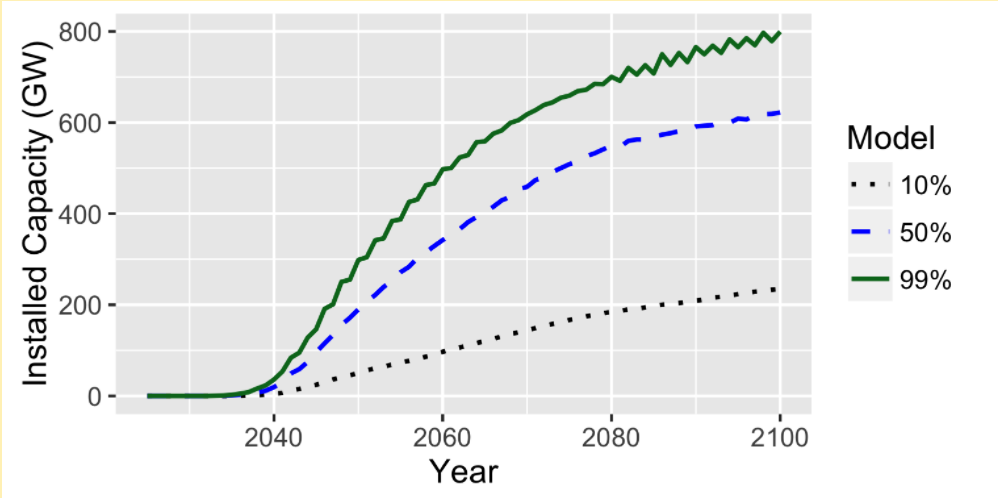
\includegraphics[width=\textwidth]{Fig4_4.png}
\end{center}
\caption{Nominal growth of fusion installed capacity at three different market capture ceilings. Each curve assumes initial fusion readiness in 2030 with a 10-year s-curve climb towards the applicable ceiling.}
\label{fig:installed_capacity}
\end{figure}

Given the granularity of the agent-based approach, one can also closely examine the gradual introduction of fusion power plants during the early years of availability. Early market capture results are summarized in Table 2.

\begin{table}[!htbp]
	\centering
	\scriptsize
	\caption{Fusion capacity additions under varying market entry years and capture limits.}
	\label{tNomenclature}
	\begin{tabular}{cccc}
Year-Limit & $M_{fus}^{t+5}$ - $M_{fus}^{t+10}$ (GW) & $M_{fus}^{2100}$ (GW) & Years until $M_{fus}^t$ $\geq$ 100 GW \\ \hline \hline
2030-10 & 0 $\vert$ 4.7 	& 230 &  31 \\
2030-50 & 1.2 $\vert$ 19.4	& 620 &  16 \\
2030-99 & 2.5 $\vert$ 36.0 	& 800 &  14 \\ \hline
2050-10 & 0.9 $\vert$ 11.7 	& 200 &  28 \\
2050-50 & 5.0 $\vert$ 51.2	& 600 &  13 \\ \hline
2070-10 & 1.0 $\vert$ 12.8 	& 120 &  26 \\
2070-50 & 5.9 $\vert$ 57.3	& 430 &  13 \\ \hline
	\end{tabular}
\end{table}


For the model to field a fusion power plant, there must be sufficiently large new capacity requirements combined with sufficient fusion technical learning, modeled by the s-curve. In the current approach, the s-curve is a proxy for growing industry capability that eventually levels off to a steady-state market capture ceiling. In some cases, even though fusion is technically available to enter the market, the product of new capacity requirements and technical readiness is insufficient to allow the model to build a new fusion power plant (denoted by the many zeros in Table 2). Generally, entering the market in later years provides a larger initial opportunity, primarily because annual electricity demand is assumed to grow over time. Another notable result is the time required to reach 100 GW of installed fusion capacity, or approximately 10\% of the current installed capacity in the United States. If fusion reaches only a 10\% market ceiling, then it will take nearly 3 decades to reach 100 GW. If fusion power plants capture up to 50\% of new capacity, however, fusion can field 100 GW of capacity within just over 1 decade. Given that some business valuation approaches make use of discounted cash flows, results such as these can help fusion companies generate the potential sales figures used in valuation calculations.

\subsection{Carbon budget threshold analysis with fusion technology present}

Another potential application of the agent-based model is to evaluate the potential for fusion power plant entry to mitigate greenhouse gas emissions by the power sector. We believe that this analysis is perhaps the most valuable to consider when considering implementation of the Green New Deal. In this scenario, the model is employed to evaluate the year the U.S. power sector will exceed a given budget for $CO_2$ equivalent emissions for various fusion power plant scenarios. According to the IPCC \citep{IPCC2014}, the world has a collective carbon budget of approximately 490 gigatonnes (Gt) of CO2 equivalent ($CO_2eq$). If global emissions exceed the budget, mitigating global mean temperature rise will become increasingly difficult. In 2014, the United States accounted for approximately 15\% of global emissions \citep{Boden2017}, of which approximately 30\% \citep{EPA2017} came from the power sector. For the purposes of this analysis, a conservative budget of 75 Gt $CO_2eq$ was allotted to the U.S. power sector. This quantity reflects an assumption that electricity will serve an increasing role in transportation in the future.

Model results for carbon budget tracking are shown in Figure \ref{fig:co2budget}. In the business-as-usual case (no fusion), the model predicts a 75 Gt $CO_2eq$ budget will be exceeded by the U.S. power sector by approximately 2055. Introducing 10\% or 50\% of new electricity procurement from fusion with a ten-year ramp-up beginning in 2030 delays exceeding this threshold by at most seven years. This modest extension indicates that total fleet-wide emissions, especially from growth in natural gas generation, will remain significant even as zero-carbon sources of electricity gain market share. Only in the extreme case where 99\% of new generation is procured from fusion power plants beginning with market entry in 2030 is there a significant extension; the carbon budget would not be exceeded until 2100, by which point annual emissions from the U.S. power sector would be approximately 99\% less than 2014 levels. For comparison, we also assessed a case where 99\% of new generation is procured from fusion power plants beginning with market entry in 2040, finding an extension of only seven years relative to the business as usual case. \emph{Thus, for fusion to have a significant impact on extending the U.S. carbon budget, it needs to achieve remarkable success in terms of both early readiness (by 2030) and near-total market capture.}

\begin{figure}
\begin{center}
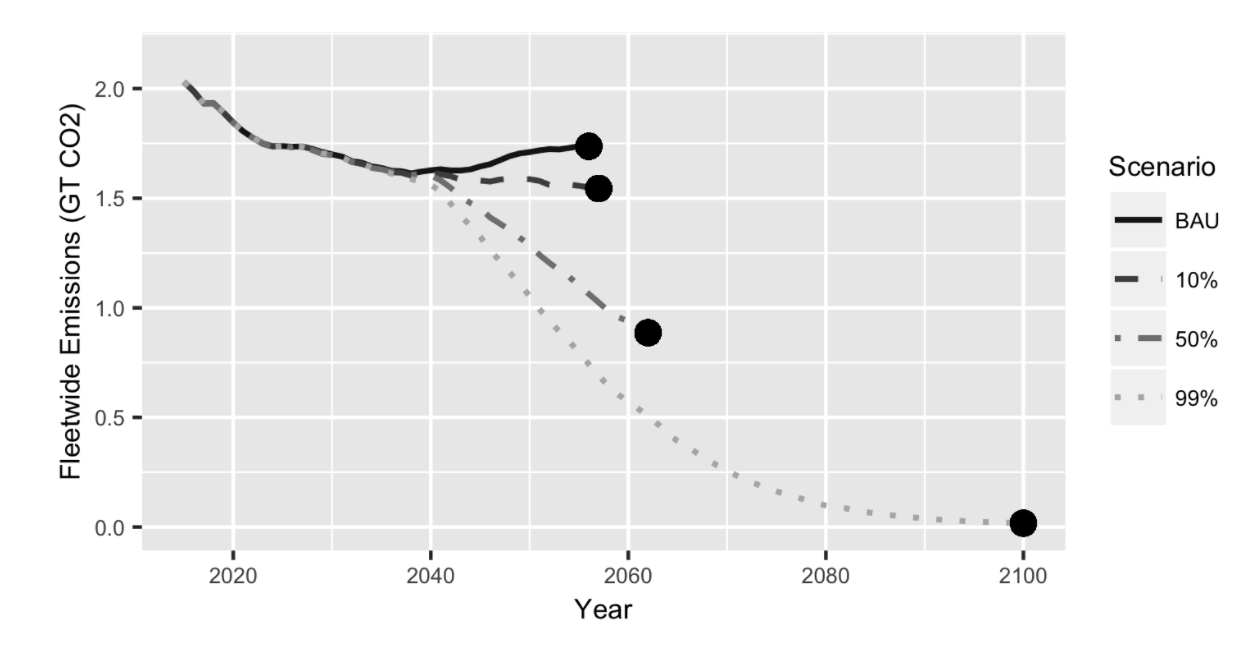
\includegraphics[width=\textwidth]{Fig4_5.png}
\end{center}
\caption{Building fusion power plants can mitigate fleet-wide carbon emissions, delaying when the fleet surpasses a 75 Gt $CO_2eq$ budget ($t_b$). Larger market penetrations for fusion delay exceeding the threshold from 2055 (BAU) to 2062 (fusion = 50\% of new energy) to 2100 (99\%). In all cases, fusion power plants become available in 2030 with a 10-year ramp-up.}
\label{fig:co2budget}
\end{figure}

\section{Limitations and Future Work}

Projections about the future composition of the U.S. generation fleet beyond current investments are dependent on numerous assumptions. Several important factors include total electricity demand over time, technology specific installed costs ($\frac{\$}{kW}$), fuel costs, national policy, distributed generation, and the evolution of the electric utility business model. This paper explores general scenarios where overall electricity demand from the grid continues to increase over time, the great majority of consumers buy electricity from the grid (as opposed to generating their own), and where national policy supports the adoption of fusion technology when it enters the market. This model discussed in this paper also does not present results from the simulation as optimal arrangements of the generation fleet. 

Geographic dispersion of the existing power plant fleet is not considered by the model. This omission is limiting because the generation fleet will evolve differently across the country. In future work, the country will be divided into four regions and power plant agents will be tracked with spatial coordinates. The model will be updated to include the cost of building new transmission if new capacity is built in areas without existing generation infrastructure. In future work, storage will be incorporated as a mitigating asset to accommodate high penetrations of non-dispatchable resources.

This model assumes that power plant agents operate at a constant capacity factor each year, and does not account for electricity market dynamics requiring that electricity supply and demand are balanced on a daily or even hourly basis. For example, growing wind and solar output might be increasingly curtailed in the future due to congestion on the transmission grid, effectively lowering their capacity factor. Sustained low natural gas prices could result in increased capacity factors from NGCC plants functioning as baseload resources. Breakthroughs in electricity storage could diminish the need for NGCT peaking plants, which typically only operate during peak demand periods. These examples serve to communicate significant uncertainties pertaining to the future of the electric grid, which ultimately frame the initial results from the model. In future work, additional sensitivity analysis of model parameters will be performed to better estimate the uncertainty in the results.

\section{Conclusion}

This study develops an agent-based model to investigate the potential for fusion power plants to capture market share within the electric sector in the United States for a range of scenarios covering technical readiness and rates of market capture. The model represents the entire grid-scale fleet, simulating retirements based on technology-specific lifetime probability distributions. The model compares well to EIA simulations for a business-as-usual case, and finds significant potential for fusion power plants to gain market share by replacing end-of-lifetime power plants. However, the ability of new fusion power plants to rapidly decarbonize the power sector is limited, even for scenarios where the technology becomes commercially viable in 2030, suggesting that early retirements might be required to keep power sector emissions below a predefined budget in the next half-century. To the best of the authors' knowledge, this work is the first time an agent-based model has been applied to simulating fusion power market entry; the results, however, agree qualitatively with other well-established energy market modeling tools \citep{ACFD}.

\section{Acknowledgements}

The authors would like to acknowledge Dr.s Colleen Nehl and Ann Xu for their comments and suggestions. The authors would additionally like to thank ARPA-E for financial support throughout the duration of the study. 


\section{Appendix}


\subsection{Comparison to EIA projections for installed capacity}

Validating the accuracy of the model during fleet-wide retirements and replacement new generation is difficult. The backbone of the model ensures sufficient capacity is built to meet total annual energy demand from the grid (measured in MWh, for example). Depending on the mix of technologies, the model adds varying amounts of installed capacity (measured in MW, for example) depending on the capacity factor of each technology.

To assess model performance in a business-as-usual scenario, its results for total capacity are compared to fleet wide capacity projections from AEO 2017 \citep{NEMS2014}  in Figure \ref{fig:EIA_comparison}. In general, there is close agreement over time, although the agent-based model exhibits some year-to-year spikes and valleys that are not seen in the AEO projection.

\begin{figure}[!htp]
\begin{center}
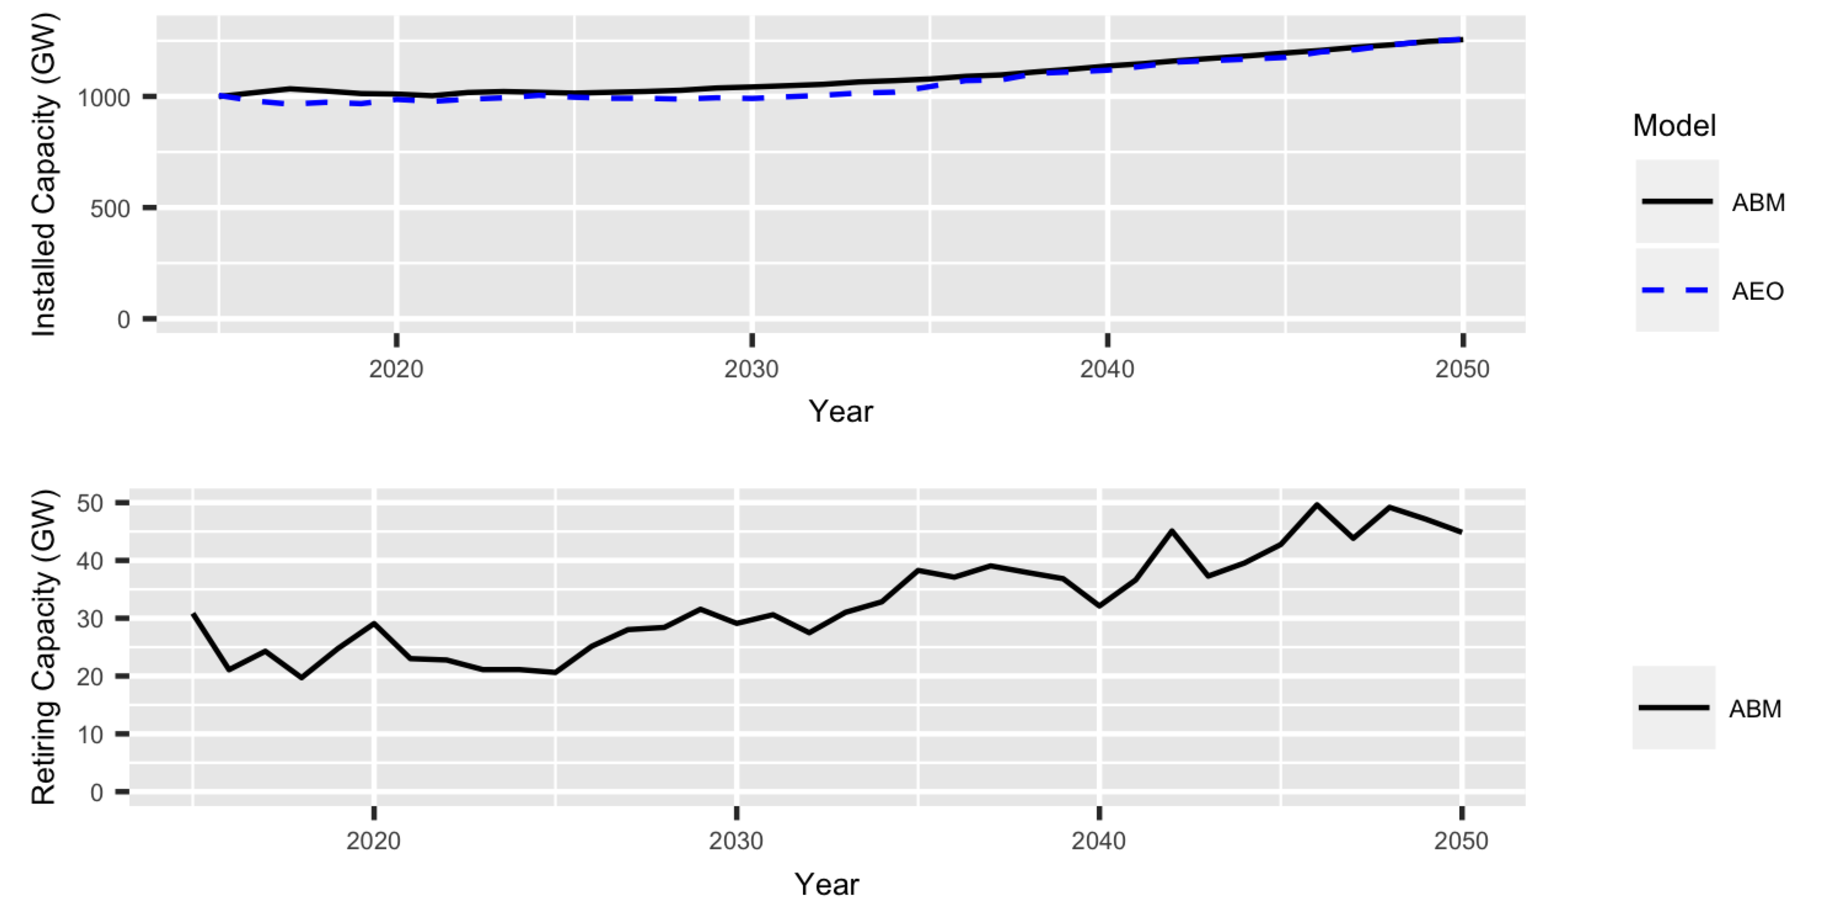
\includegraphics[width=\textwidth]{Fig4_1.png}
\end{center}
\caption{Top: Agent-based model (ABM) projections for total installed capacity on the grid compared to EIA projections. Bottom: model projections for annual capacity retirements of all types. The modeled installed capacity tracks EIA numbers closely, while annual retirements generally climb as capacity grows.}
\label{fig:EIA_comparison}
\end{figure}

\subsection{Capacity by generation fuel type in business as usual scenario}


According to EIA projections, 86\% of new capacity added to the grid before 2050 will come from NGCC, wind, photovoltaics, or other renewables; and installed capacity from coal, petroleum, NGST, and nuclear fission will decrease from 450 GW in 2017 to 270 GW in 2050 as existing power plants are retired and not replaced, excepting approximately 4.4 GW of nuclear capacity currently under construction \citep{NEMS2014} . Model results for grid capacity by generation type in the absence of fusion technology are shown in Figure \ref{fig:without_nuclear}. In general, the model finds that in the absence of fusion technology, grid capacity in 2050 will be dominated by natural gas technologies, although wind and solar capacity will nearly triple over the same period.

Qualitatively, these results resemble those published in the AEO 2017 \citep{NEMS2014} , although the model finds much faster growth in natural gas combined cycle and combustion turbine capacity relative to AEO projections. For example, the model anticipates NGCC and NGCT capacity on the grid will be approximately 680 GW in 2050, over half of the total installed capacity, whereas the EIA projects only 521 GW of NGCC and NGCT capacity in 2050. In general, model results predict natural gas capacity in 2050 will be primarily NGCC, largely due to its representation of mean lifetime in the model, which exceeds the mean lifetime of combustion turbines. The model shows good agreement with EIA data on renewable projections (including conventional hydro, geothermal, and biomass), projecting 471 GW of installed capacity in 2050 compared to AEO's projection of 432 GW.

Based on the retirement age of the existing fleet and the methods used to project plant retirements, the model predicts a more rapid decline of coal, natural gas steam, and nuclear generation capacity relative to AEO data. For example, the model projects there will only be 43 GW of coal capacity on the grid in 2050, compared to an AEO projection of 157 GW. Similarly, nuclear capacity in the model declines to 8 GW in 2040, compared to an AEO projection of 77 GW. This difference potentially reflects an AEO assumption that most nuclear power plants will continue operating beyond 2050, irrespective of current license expirations.

\begin{figure}
\begin{center}
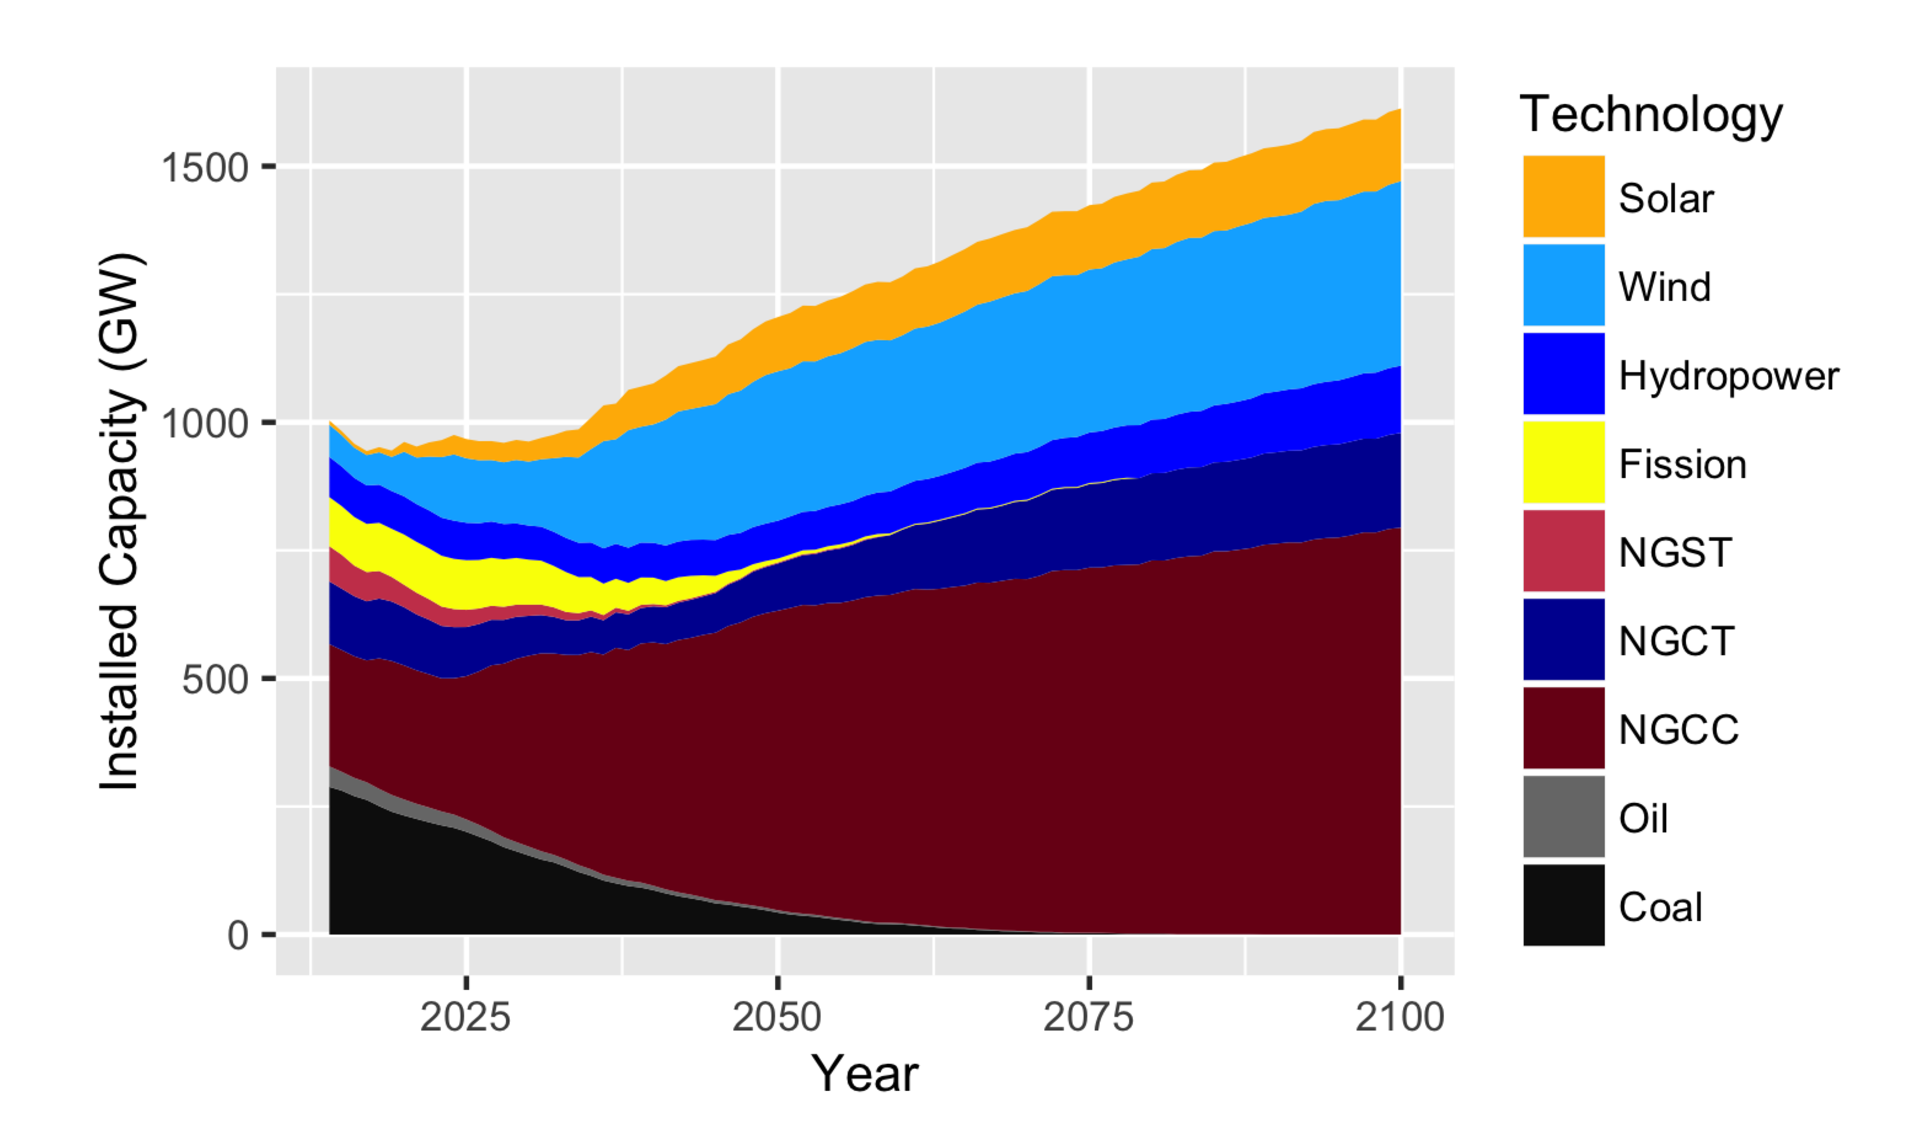
\includegraphics[width=\textwidth]{Fig4_2.png}
\end{center}
\caption{Model projections for total installed grid-scale capacity by fuel type according to EIA projections. The majority of growth comes from NGCC, wind, and photovoltaics. Contributions from coal, nuclear, petroleum, and NGST are expected to diminish while hydro and NGCT remain roughly constant.}
\label{fig:without_nuclear}
\end{figure}

Beyond 2050, the model predicts that existing capacity will increasingly be replaced by new capacity as the existing fleet is retired and new generators are built. Figure 3 shows model projections for total installed capacity and cumulative new capacity as well as for cumulative capacity additions, all of which can help describe the approximate size of the market opportunity for new power plants. The model predicts that by 2050 the total installed capacity on the grid will be 1250 GW, of which 1050 GW will be built between 2014 and 2050. By approximately 2075, 99\% of the total capacity on the grid will have been constructed after 2014. The rate of new construction is driven by model projections for power plant retirements, which depends on the life expectancy for each power plant agent in the model. Qualitatively, these results suggest the market opportunity for new types of generation will be greatest before 2050, although several hundred GW of new capacity will still need to be built in the second half of the century. Nevertheless, Figure 3 also shows that the majority of new plants result from a need to replace retiring capacity, with only a small fraction of the new additions being driven by electricity demand growth.

\begin{figure}
\begin{center}
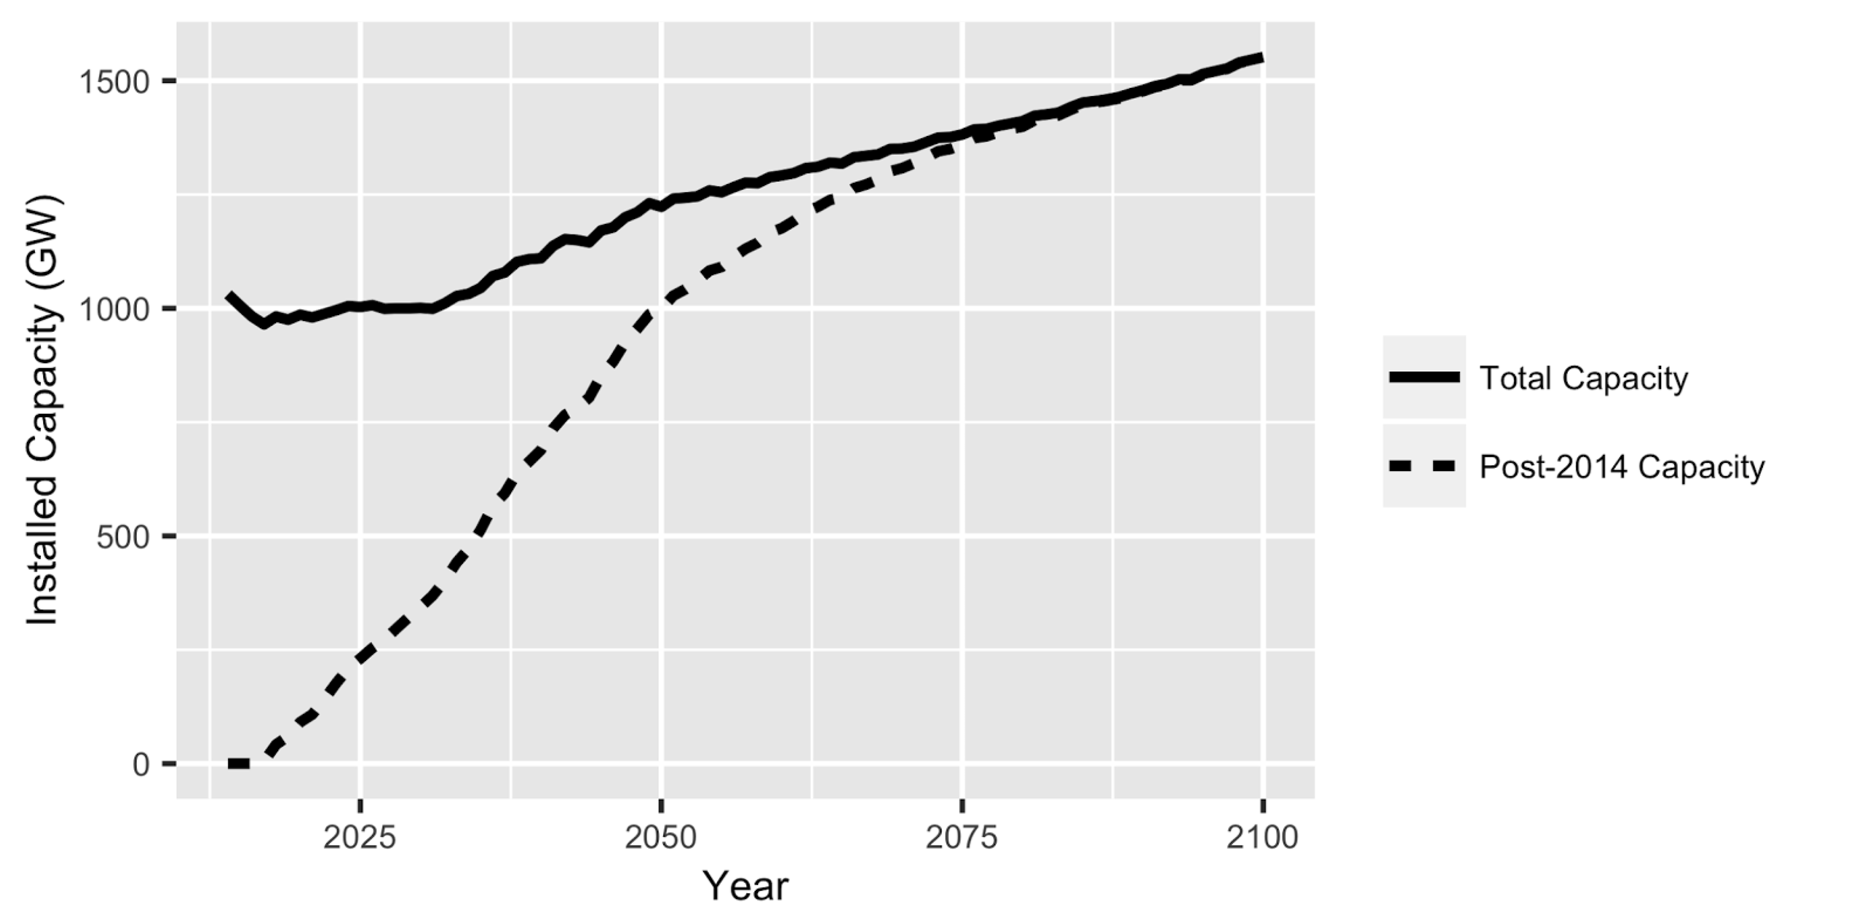
\includegraphics[width=\textwidth]{Fig4_2b.png}
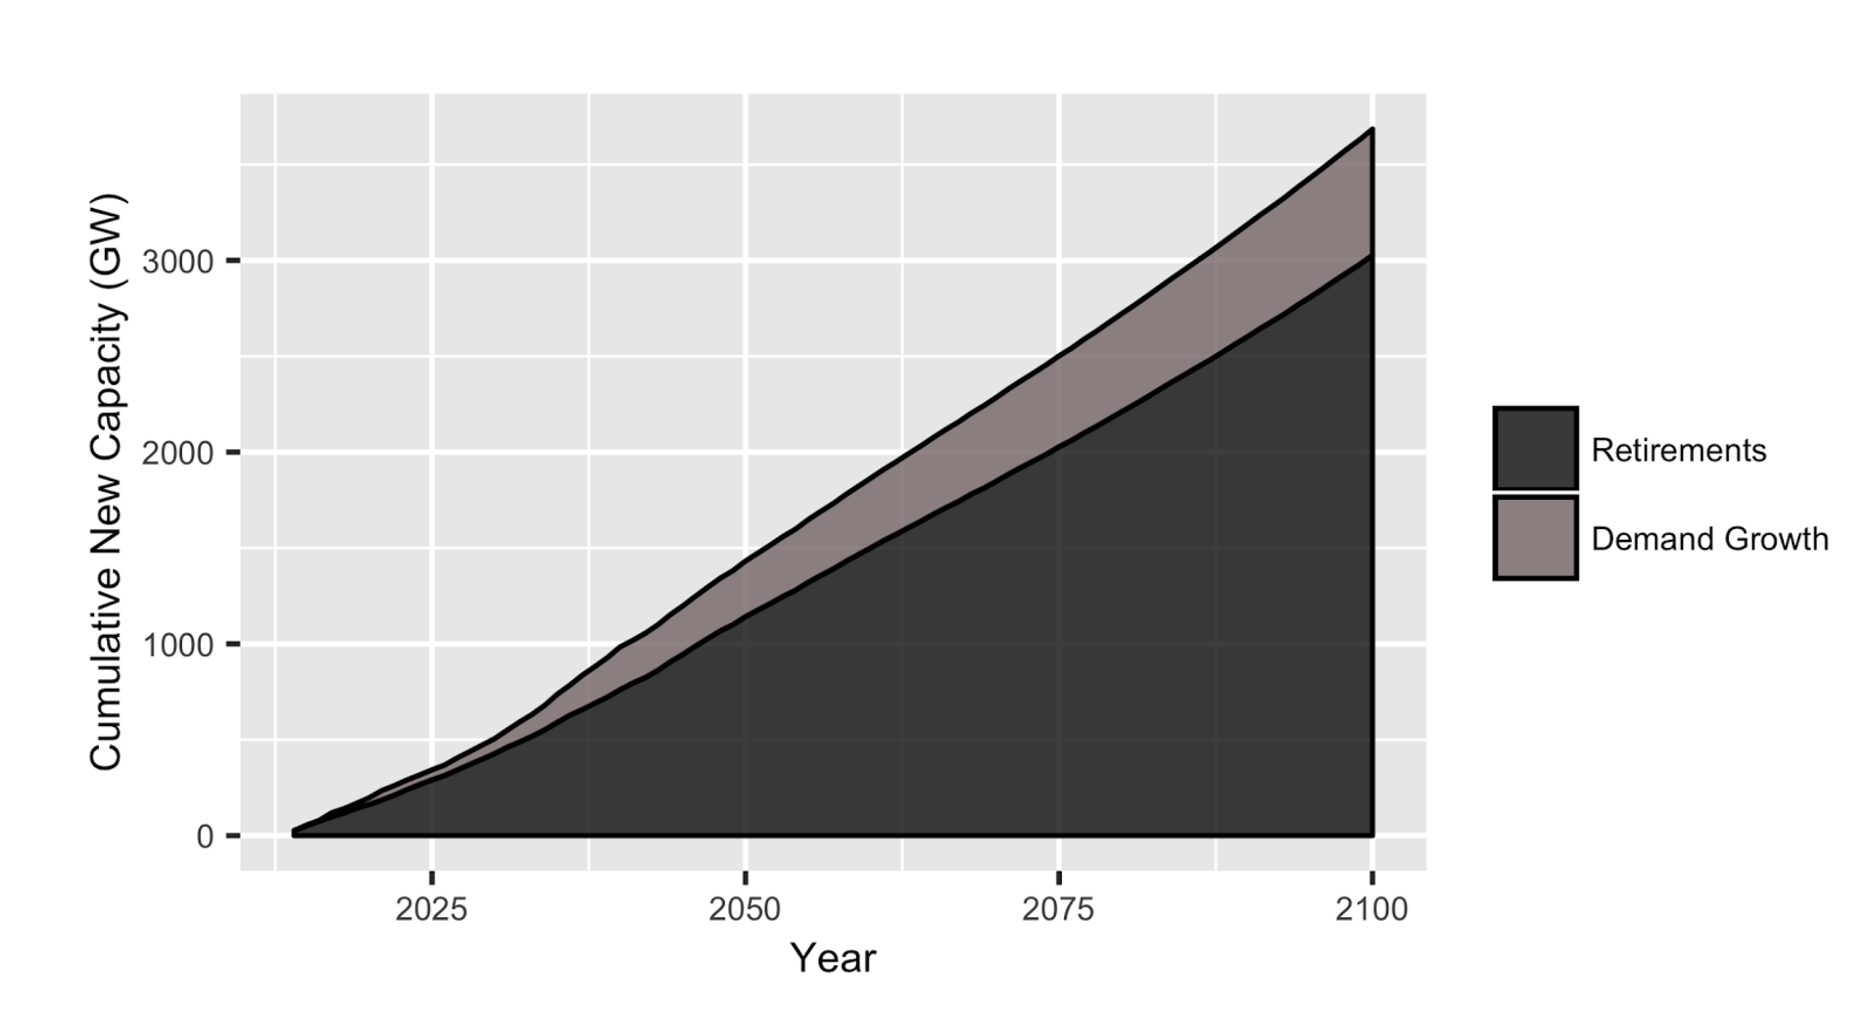
\includegraphics[width=\textwidth]{Fig4_3.png}
\end{center}
\caption{Above, model predictions for total installed capacity and cumulative new capacity added after 2014. The rate of new capacity construction slows beyond 2050. Below, the primary driver of new construction is retiring capacity rather than electricity demand growth}
\end{figure}


\newpage

\nocite{*}

\section{References}

\bibliography{alpha1}

\end{document}
